\chapter{运输层}

    运输层位于应用层和网络层之间,是分层的网络体系结构的重要部分。该层为运行在不同主机上的应用进程提供直接的通信服务起着至关重要的作用。

\section{概述和运输层服务}

    运输层协议为运行在不同主机上的应用进程之间提供了逻辑通信(logic communication)功能。从应用程序的角度看,通过逻辑通信,运行不同进程的主机好像直接相连一样;

\begin{figure}[!htbp]
    \centering
    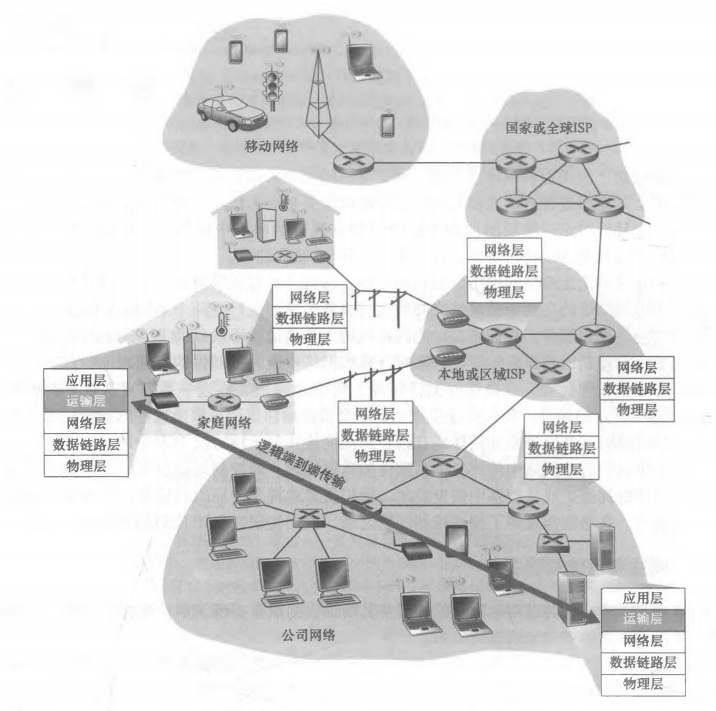
\includegraphics[width=0.6\textwidth]{image/chapter03/运输层.png}
    \caption{运输层在应用程序进程间提供逻辑的并非物理的通信}
\end{figure}

    如上图所示,运输层协议是在端系统中而不是在路由器中实现的。在发送端,运输层将从发送应用程序进程接收到的报文转换成运输层分组,用因特网术语来讲该分组称为运输层报文段(segment)。

    实现的方法(可能)是将应用报文划分为较小的块,并为每块加上一个运输层首部以生成运输层报文段。然后,在发送端系统中,运输层将这些报文段传递给网络层,网路层将其封装成网络层分组(即数据报)并向目的地发送。

\subsection{运输层和网络层的关系}

    网络层提供了主机之间的逻辑通信,而运输层为运行在不同主机上的进程之间提供了逻辑通信。

    运输层协议只工作在端系统中。在端系统中,运输层协议将来自应用进程的报文移动到网络边缘(即网络层),反过来也是一样,但对有关这些报文在网络核心如何移动并不作任何规定。

    运输协议能够提供的服务常常受制于底层网络层协议的服务模型。如果网络层协议无法为主机之间发送的运输层报文段提供时延或带宽保证的话,运输层协议也就无法为进程之间发送的应用程序报文提供时延或带宽保证。

\subsection{因特网运输层概述}

    因特网为应用层提供了两种截然不同的可用运输层协议。这些协议一种是UDP(用户数据报协议),它为调用它的应用程序提供了一种不可靠、无连接的服务。另一种是TCP(传输控制协议),它为调用它的应用程序提供了一种可靠的、面向连接的服务。

    为了简化术语,我们将运输层分组称为报文段(segment)。然而,\emph{因特网文献(如RFC文档)也将TCP的运输层分组称为报文段,而常将UDP的分组称为数据报(data gram)。而这类因特网文献也将网络层分组称为数据报!}在此处,我们将TCP和UDP的分组统称为报文段。

    因特网网络层协议有一个名字叫IP,即网际协议。IP为主机之间提供了逻辑通信。IP的服务模型是尽力而为交付服务(best-effort delivery service)。

    这意味着IP尽它“最大的努力”在通信的主机之间交付报文段,但它并不做任何确保。特别是,它不确保报文段的交付,不保证报文段的按序交付,不保证报文段中数据的完整性。由于这些原因,IP被称为不可靠服务(unreliable service)。在此处,我们只需要记住每台主机只有一个IP地址。

    UDP和TCP最基本的责任是,将两个端系统间IP的交付服务扩展为运行在端系统上的两个进程之间的交付服务。将主机间交付扩展到进程间交付被称为运输层的多路复用(transport-layer multiplexing)与多路分解(demultiplexing)。

    UDP和TCP还可以通过在其报文段首部中包括差错检查字段而提供完整性检查。进程到进程的数据交付和差错检查是两种最低限度的运输层服务,也是UDP所能提供的仅有的两种服务。特别是,与IP—样,UDP也是一种不可靠的服务,即不能保证一个进程所发送的数据能够完整无缺地(或全部!)到达目的进程。

\section{多路复用与多路分解}

    \emph{多路复用与多路分解服务是所有计算机网络都需要的}。

    在目的主机,运输层从紧邻其下的网络层接收报文段。运输层负责将这些报文段中的数据交付给在主机上运行的适当应用程序进程。

    一个进程(作为网络应用的一部分)有一个或多个套接字(socket),它相当于从网络向进程传递数据和从进程向网络传递数据的门户。因此,如下所示,在接收主机中的运输层实际上并没有直接将数据交付给进程,而是将数据交给了一个中间的套接字。由于在任一时刻,在接收主机上可能有不止一个套接字,所以每个套接字都有唯一的标识符。

\begin{figure}[!htbp]
    \centering
    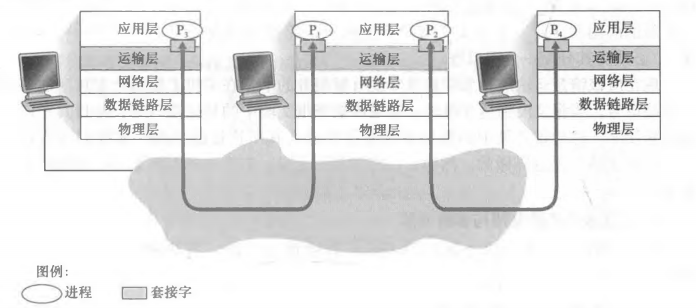
\includegraphics[width=0.6\textwidth]{image/chapter03/多路复用和多路分解.png}
    \caption{运输层的多路复用与多路分解}
\end{figure}

    现在我们考虑接收主机怎样将一个到达的运输层报文段定向到适当的套接字。为此目的,每个运输层报文段中具有几个字段。在接收端,运输层检查这些字段,标识出接收套接字,进而将报文段定向到该套接字。

    \emph{将运输层报文段中的数据交付到正确的套接字}的工作称为多路分解(demultiplexing)。

    \emph{在源主机从不同套接字中收集数据块,并为每个数据块封装上首部信息(这将在以后用于分解)从而生成报文段,然后将报文段传递到网络层,所有这些工作}称为多路复用(multiplexing)。

    运输层多路复用要求:

\begin{itemize}
    \item [1)] 套接字有唯一标识符
    \item [2)] 每个报文段有特殊字段来指示该报文段所要交付到的套接字
\end{itemize}

\begin{figure}[!htbp]
    \centering
    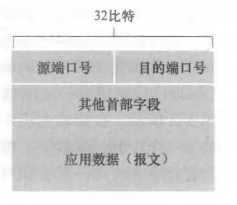
\includegraphics[width=0.4\textwidth]{image/chapter03/运输层报文段中的源-目的端口号字段.png}
    \caption{运输层报文段中源与目的端口字段}
\end{figure}

    这些特殊字段是源端口号字段(source port number field)和目的端口号字段(destination port number field)。

    端口号是一个16比特的数,其大小在0 ~ 65535之间。0 ~ 1023范围的端口号称为周知端口号(well-known port number),是受限制的。

    现在应该清楚运输层是怎样能够实现分解服务的了:在主机上的每个套接字能够分配一个端口号,当报文段到达主机时,运输层检査报文段中的目的端口号,并将其定向到相应的套接字。然后报文段中的数据通过套接字进入其所连接的进程。

\subsubsection{无连接的多路复用与多路分解}

    \emph{一个UDP套接字是由一个二元组全面标识的,该二元组包含一个目的IP地址和一个目的端口号。因此,如果两个UDP报文段有不同的源IP地址和/或源端口号,但具有相同的目的IP地址和目的端口号,那么这两个报文段将通过相同的目的套接字被定向到相同的目的进程}

\subsubsection{面向连接的多路复用和多路分解}

    \emph{TCP套接字是由一个四元组(源IP地址, 源端口号,目的IP地址,目的端口号)来标识的。因此,当一个TCP报文段从网络到达一台主机时,该主机使用全部4个值来将报文段定向(分解)到相应的套接字。特别与UDP不同的是,两个具有不同源IP地址或源端口号的到达TCP报文段将被定向到两个不同的套接字,除非TCP报文段携带了初始创建连接的请求}。

\section{无连接运输:UDP}

    由[RFC 768]定义的UDP只是做了运输协议能够做的最少工作。除了复用/分解功 能及少量的差错检测外,它几乎没有对IP增加别的东西。

    有许多应用更适合用UDP,原因主要以下几点:

\begin{itemize}
    \item [1)] 关于发送什么数据以及何时发送的应用层控制更为精细。
    \subitem 采用UDP时,只要应用进程将数据传递给UDP, UDP就会将此数据打包进UDP报文段并立即将其传递给网络层。
    \item [2)] 无须连接建立。
    \subitem UDP不会引入建立连接的时延。这可能是DNS运行在UDP之上而不是运行在TCP之上的主要原因。
    \item [3)] 无连接状态。
    \subitem TCP需要在端系统中维护连接状态。此连接状态包括接收和发送缓存、拥塞控制参数以及序号与确认号的参数。UDP不维护连接状态,也不跟踪这些参数。
    \item [4)] 分组首部开销小。
    \subitem 每个TCP报文段都有20字节的首部开销,而UDP仅有8字节的开销。
\end{itemize}

\subsection{UDP报文段结构}

\begin{figure}[!htbp]
    \centering
    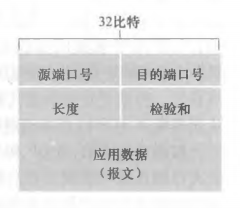
\includegraphics[width=0.4\textwidth]{image/chapter03/UDP报文段结构.png}
    \caption{UDP报文段结构}
\end{figure}

    UDP首部只有4个字段,每个字段由两个字节组成。通过端口号可以使目的主机将应用数据交给运行在目的端系统中的相应进程(即执行分解功能)。长度字段指示了在UDP报文段中的字节数(首部加数据)。因为数据字段的长度在一个UDP段中不同于在另一个段中,故需要一个明确的长度。接收方使用检验和来检查在该报文段中是否出现了差错。

\subsection{UDP校验和}

    UDP检验和提供了差错检测功能。这就是说,检验和用于确定当UDP报文段从源到达目的地移动时,其中的比特是否发生了改变。

    发送方的UDP对报文段中的所有16比特字的和进行反码运算, 求和时遇到的任何溢出都被回卷。得到的结果被放在UDP报文段中的检验和字段。

    在既无法确保逐链路的可靠性,又无法确保内存中的差错检测的情况下,如果端到端数据传输服务要提供差错检测,UDP就必须在端到端基础上在运输层提供差错检测。这是一个在系统设计中被称颂的端到端原则(end-encl principle)的例子。

\section{可靠数据传输原理}

    下图说明了我们的学习框架。为上层实体提供的服务抽象是:数据可以通过一条可靠的信道进行传输。借助于可靠信道,传输数据比特就不会受到损坏(由0变为1,或者相反)或丢失,而且所有数据都是按照其发送顺序进行交付。这恰好就是TCP向调用它的因特网应用所提供的服务模型。

\begin{figure}[!htbp]
    \centering
    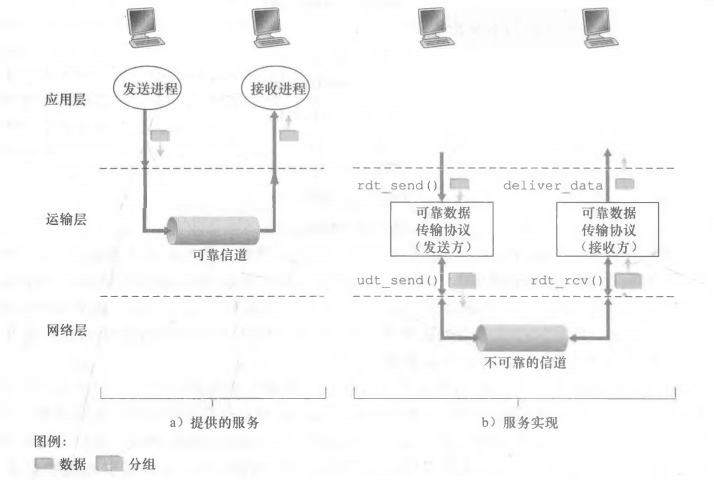
\includegraphics[width=0.6\textwidth]{image/chapter03/可靠数据传输.png}
    \caption{可靠数据传输:服务模型与服务实现}
\end{figure}

    实现这种服务抽象是可靠数据传输协议(reliable data transfer protocol)的责任。由于可靠数据传输协议的下层协议也许是不可靠的,因此这是一项困难的任务。

\subsection{构造可靠数据传输协议}

\subsubsection{经完全可靠信道的可靠数据传输:rdt1.0}

    首先,我们考虑最简单的情况,即底层信道是完全可靠的。我们称该协议为rdt1.0,该协议本身是简单的。

\begin{figure}[!htbp]
    \centering
    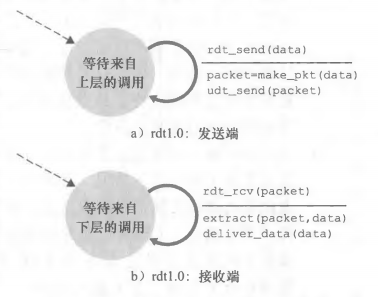
\includegraphics[width=0.6\textwidth]{image/chapter03/rdt1.0-用于完全可信的数据传输.png}
    \caption{rdt1.0:用于完全可靠信道的协议}
\end{figure}

    上图显示了rdt1.0发送方和接收方的有限状态机(Finite-State Machine, FSM)的定义。

    发送方和接收方有各自的FSM。上图中发送方和接收方的FSM每个都只有一个状态。FSM描述图中的箭头指示了协议从一个状态变迁到另一个状态(因为每个FSM都只有一个状态,因此变迁必定是从一个状态返回到自身;我们很快将看到更复杂的状态图)。

    引起变迁的事件显示在表示变迁的横线上方,事件发生时所采取的动作显示在横线下方。如果对一个事件没有动作,或没有事件发生而采取了一个动作,我们将横线上方或下方使用符号$\land$,以分别明确地表示缺少动作或事件。FSM初始状态用虚线表示。

\subsubsection{经具有比特差错信道的可靠数据传输:rdt2.0}

    底层信道更为实际的模型是分组中的比特可能受损的模型。在分组的传输、传播或缓存的过程中,这种比特差错通常会岀现在网络的物理部件中。

    在研发一种经这种信道进行可靠通信的协议之前,首先考虑一下人们会怎样处理这类情形。种口述报文协议使用了肯定确认(positive acknowledgment)("OK”)与否定确认(negative acknowledgmenl)("请重复一遍)。这些控制报文使得接收方可以让发送方知道哪些内容被正确接收,哪些内容接收有误并因此需要重复。在计算机网络环境中,基于这样重传机制的可靠数据传输协议称为自动重传请求 (Automatic Repeat reQuest, ARQ)协议。

    ARQ协议中需要另外三种协议来处理存在比特差错的情况:

\begin{itemize}
    \item [1)] 差错检测。
    \subitem 首先,需要一种机制以使接收方检测到何时出现了比特差错。前一节讲到,UDP使用因特网检验和字段正是为了这个目的。
    \item [2)] 接收方反馈。
    \subitem 因为发送方和接收方通常在不同端系统上执行,可能相隔数千英里, 发送方要了解接收方情况(此时为分组是否被正确接收)的唯一途径就是让接收方提供明确的反馈信息给发送方。我们的rdt2.0协议将从接收方向发送方回送ACK与NAK分组。理论上,这些分组只需要一个比特长; 如用0表示NAK,用1表示ACK。
    \item [3)] 重传。
    \subitem 接收方收到有差错的分组时,发送方将重传该分组文。
\end{itemize}

\begin{figure}[!htbp]
    \centering
    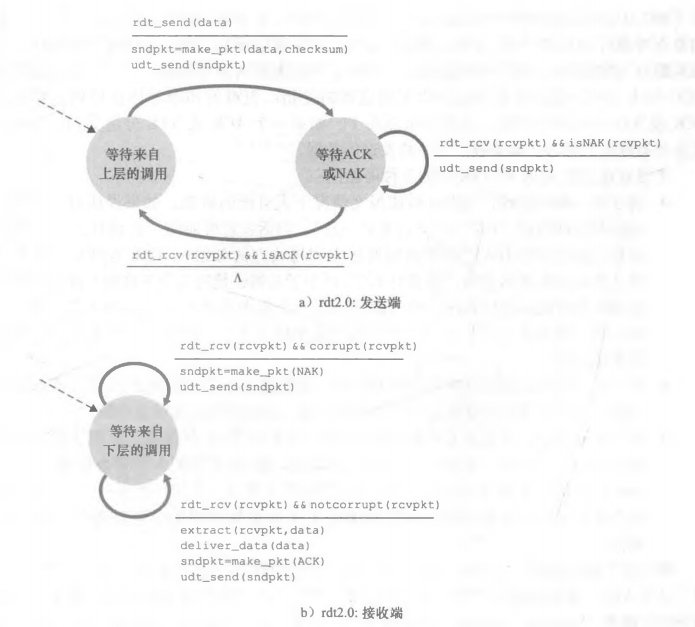
\includegraphics[width=0.6\textwidth]{image/chapter03/rdt2.0-具有比特差错的机制.png}
    \caption{rdt2.0:用于具有比特差错信道的协议}
\end{figure}

    下图表示rdt2.0的FSM,该数据协议采用了差错检测、肯定确认与否定确认。

    rdt2.0的发送端有两个状态。在最左边的状态中,发送端协议正等待来自上层传下来的数据。当$rdt\_send(data)$事件岀现时,发送方将产生一个包含待发送数据的分组(sndpkt),带有检验和,然后经由$udt\_send(sndpkt)$操作发送该分组。

    在最右边的状态中,发送方协议等待来自接收方的ACK或NAK分组。如果收到一个ACK分组(图中符号$rdt\_rcv(rcvpkt) \&\& isACK(rcvpkt)$对应该事件),则发送方知道最近发送的分组已被正确接收,因此协议返回到等待来自上层的数据的状态。如果收到一个NAK分组,该协议重传上一个分组并等待接收方为响应重传分组而回送的ACK和NAK。

    \emph{当发送方处于等待ACK或NAK的状态时,它不能从上层获得更多的数据;这就是说,rdcsend()事件不可能岀现;仅当接收到ACK并离开该状态时才能发生这样的事件。因此,发送方将不会发送一块新数据,除非发送方确信接收方已正确接收当前分组}。由于这种行为,rdt2.0这样的协议被称为停等(stop and-wait)协议

    rdt2.0协议看起来似乎可以运行了,但遗憾的是,它存在一个致命的缺陷。尤其是我们没有考虑到ACK或NAK分组受损的可能性!

    考虑处理ACK和NAK时的三种可能性:

\begin{itemize}
    \item [1)] 第一种可能性,接收者不明白发起者的话是口述内容的一部分还是一个要求重复上次回答的请求
    \item [2)] 第二种可能性,增加足够的检验和比特,使发送方不仅可以检测差错,还可恢复差错。对于会产生差错但不丢失分组的信道,这就可以直接解决问题
    \item [3)] 第三种方法是,当发送方收到含糊不清的ACK或NAK分组时,只需重传当前数据分组即可。
    \subitem 这种方法在发送方到接收方的信道中引入了冗余分组(duplicate packet)。冗余分组的根本困难在于接收方不知道它上次所发送的ACK或NAK是否被发送方正确地收到。因此它无法事先知道接收到的分组是新的还是一次重传!
\end{itemize}

    解决这个新问题的一个简单方法(几乎所有现有的数据传输协议中,包括TCP,都采用了这种方法)是在数据分组中添加一新字段,让发送方对其数据分组编号,即将发送数据分组的序号(sequence number)放在该字段。

\begin{figure}[!htbp]
    \centering
    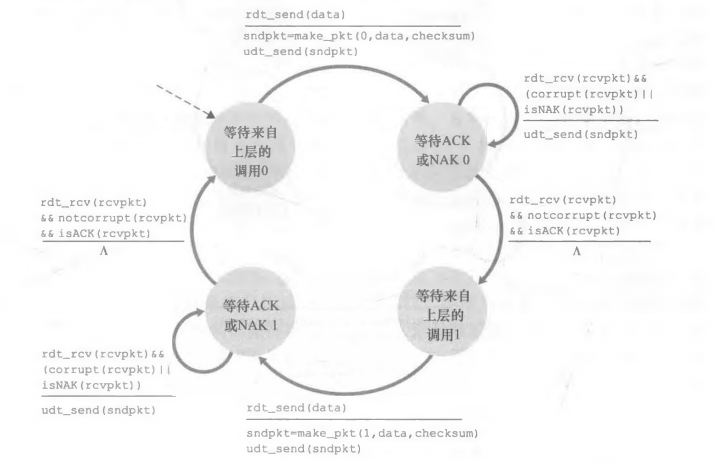
\includegraphics[width=0.6\textwidth]{image/chapter03/rdt2.1发送方.png}
    \caption{rdt2.1 发送方}
\end{figure}

\begin{figure}[!htbp]
    \centering
    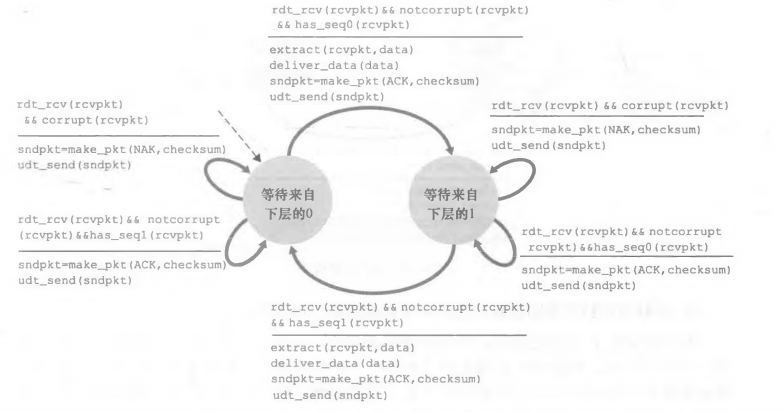
\includegraphics[width=0.6\textwidth]{image/chapter03/rdt2.1接收方.png}
    \caption{rdt2.1 接收方}
\end{figure}

    剩下的rdt2.2,rdt3.0后面再说吧。。不想看了

\section{面向连接的运输:TCP}

\subsection{TCP连接}

    TCP被称为是面向连接的(connection-oriented),这是因为在一个应用进程可以开始向另一个应用进程发送数据之前,这两个进程必须先相互“握手”,即它们必须相互发送某些预备报文段,以建立确保数据传输的参数。作为TCP连接建立的一部分,连接的双方都将初始化与TCP连接相关的许多TCP状态变量

    TCP连接也总是点对点(point-to-point)的,即在单个发送方与单个接收方之间的连接。所谓“多播”(参见本书的在线补充材料),即在一次发送操作中,从一个发送方将数据传送给多个接收方,这种情况对TCP来说是不可能的。

    一旦建立起一条TCP连接,两个应用进程之间就可以相互发送数据了。客户进程通过套接字(该进程之门)传递数据流。数据一旦通过该门,它就由客户中运行的TCP控制了。

\begin{figure}[!htbp]
    \centering
    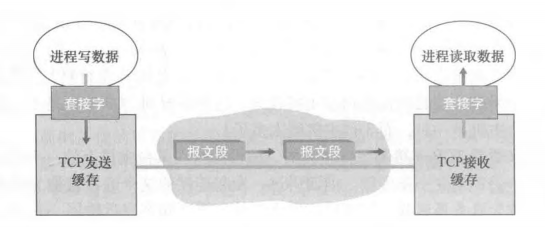
\includegraphics[width=0.6\textwidth]{image/chapter03/TCP发送缓存和接收缓存.png}
    \caption{TCP发送缓存和接收缓存}
\end{figure}

    TCP将这些数据引导到该连接的发送缓存(send buffer)里,发送缓存是发起三次握手期间设置的缓存之一。接下来TCP就会不时从发送缓存里取出一块数据,并将数据传递到网络层。

    TCP可从缓存中取出并放入报文段中的数据数量受限于最大报文段长度(Maximum Segment Size,MSS)。MSS通常根据最初确定的由本地发送主机发送的最大链路层帧长度(即所谓的最大传输单元(Maximum Transmission Unit, MTU))来设置。

    设置该MSS要保证一个TCP报文段(当封装在一个IP数据报中)加上TCP/IP首部长度(通常40字节)将适合单个链路层帧。以太网和PPP链路层协议都具有1500字节的MTU,因此MSS的典型值为1460字节。已经提出了多种发现路径MTU的方法,并基于路径MTU值设置MSS(路径MTU是指能在从源到目的地的所有链路上发送的最大链路层帧[RFC 1191])。注意到MSS是指在报文段里应用层数据的最大长度,而不是指包括首部的TCP报文段的最大长度。

\subsection{TCP报文结构}

    TCP报文段由首部字段和一个数据字段组成。数据字段包含一块应用数据。如前所述,MSS限制了报文段数据字段的最大长度。当TCP发送一个大文件,例如某Web页面上的一个图像时,TCP通常是将该文件划分成长度为MSS的若干块(最后一块除外,它通常小于MSS)。

    下图显示了TCP报文段的结构:

\begin{figure}[!htbp]
    \centering
    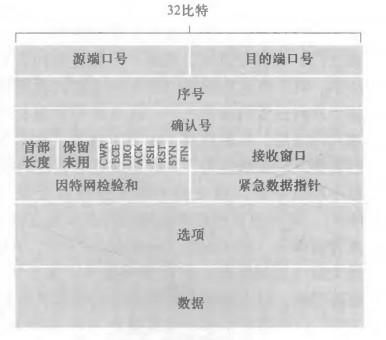
\includegraphics[width=0.6\textwidth]{image/chapter03/TCP报文结构.png}
    \caption{TCP报文段结构}
\end{figure}

    除了源端口号和目的端口号外,还包括:

\begin{itemize}
    \item [1)] 32比特的序号字段(sequence number field)和32比特的确认号字段(acknowledgment number field)
    \subitem 这些字段被TCP发送方和接收方用来实现可靠数据传输服务
    \item [2)] 16比特的接收窗口字段(receive window field)
    \subitem 该字段用于流量控制。我们很快就会看到,该字段用于指示接收方愿意接受的字节数量。
    \item [3)] 4比特的首部长度字段(header length field)
    \subitem 该字段指示了以32比特的字为单位的TCP首部长度。由于TCP选项字段的原因,TCP首部的长度是可变的。(通常,选项字段为空,所以TCP首部的典型长度是20字节。)
    \item [4)] 可选与变长的选项字段(options field)
    \subitem 该字段用于发送方与接收方协商最大报文段长度(MSS)时,或在高速网络环境下用作窗口调节因子时使用。首部字段中还定义了一个时间戳选项。
    \item [5)] 6比特的标志字段(flag field)
    \subitem [a] ACK比特用于指示确认字段中的值是有效的,即该报文段包括一个对已被成功接收报文段的确认。
    \subitem [b] RST、SYN和FIN比特用于连接建立和拆除
    \subitem [c] 在明确拥塞通告中使用了CWR和ECE比特
    \subitem [d] 当PSH比特被置位时,就指示接收方应立即将数据交给上层
    \subitem [e] URG比特用来指示报文段里存在着被发送端的上层实体置为“紧急”的数据。紧急数据的最后一个字节由16比特的紧急数据指针字段(urgent data pointer field)指出。当紧急数据存在并给出指向紧急数据尾指针的时候,TCP必须通知接收端的上层实体。
\end{itemize}

    \emph{在实践中,PSH、URG和紧急数据指针并没有使用。为了完整性起见,我们才提到这些字段}。

\subsubsection{序号和确认号}

    TCP报文段首部中两个最重要的字段是序号字段和确认号字段。这两个字段是TCP可靠传输服务的关键部分。

    TCP把数据看成一个无结构的、有序的字节流。

    假设主机A上的一个进程想通过一条TCP连接向主机B上的一个进程发送一个数据流。主机A中的TCP将隐式地对数据流中的每一个字节编号。假定数据流由一个包含500000字节的文件组成,其MSS为1000字节,数据流的首字节编号是0。如下图所示,该TCP将为该数据流构建500个报文段。给第一个报文段分配序号0, 第二个报文段分配序号1000, 第三个报文段分配序号2000, 以此类推。

\begin{figure}[!htbp]
    \centering
    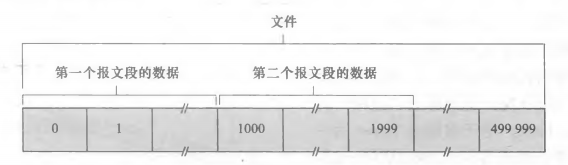
\includegraphics[width=0.6\textwidth]{image/chapter03/文件数据划分成TCP报文段.png}
    \caption{文件数据划分成TCP报文段}
\end{figure}

    现在来讨论确认号。\emph{主机A填充进报文段的确认号是主机A期望从主机B收到的下一字节的序号。}假如主机A已经收到了来自主机B的0~535的所有字节,那么如果想要接收后续的字节,主机A应该往主机B发送536的确认号。

    那么,TCP中如果数据的包有丢失(比如主机A收到了0~535与900~1000的报文段),很显然,主机A没有接收到536~899的报文段。因此,主机A需要重新构建主机B的数据流,因此A到B的下一个报文段将在确认号中包含536。\emph{因为TCP只确认该流中第一个丢失字节为止的字节,因此TCP被称为提供累计确认(cumulative acknowledgment)}。

    最后,我们来考虑:当主机在一条TCP连接中收到失序报文段时该怎么办?

\begin{itemize}
    \item [1)] 接收方立即丢弃失序报文段
    \item [2)] 接收方保留失序的字节,并等待缺少的字节以填补该间隔
\end{itemize}

    显然,第二种选择对网络贷款更为有效,是实践中采用的方法。

\subsubsection{Telnet: 序号和确认号的一个学习案例}

\begin{figure}[!htbp]
    \centering
    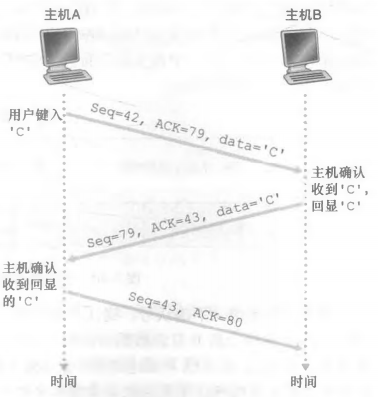
\includegraphics[width=0.6\textwidth]{image/chapter03/经TCP的简单Telnet链接.png}
    \caption{一个经TCP的简单Telnet应用的确认号和序号}
\end{figure}

    假设A发起会话(因此,主机A被标记为客户)。假设客户和服务器的起始序号分别为42和79,\emph{一个报文段的序号就是该报文段数据字段首字节的序号。确认号就是主机正在等待的数据的下一个字节序号。}

    因此,客户发送的第一个报文段序号为42,请求服务器的确认号为79。

    第二个报文段由服务器发往客户。首先为该服务器收到的数据提供一个确认,因此在确认号中填入了43,然后回显了字符'C',因此在data段中填入了字符'C'。

    \emph{值得注意的是,对客户到服务器的数据的确认被装载在一个承载服务器到客户的数据的报文段中;这种确认被称为是被捎带(piggybacked)在服务器到客户的数据报文段中的。}

    第三个报文段是从客户端发往服务器。其唯一目的是确认已从服务器收到的数据。因此确认号中填入的80.

\subsection{往返实践的估计与超时}

    \emph{TCP采用超时/重传机制来处理报文段的丢失问题。}

\subsubsection{估计往返时间}

    TCP通过如下方式估计往返时间:报文段的样本RTT(表示为SampleRTT)就是从某报文段被发出(即交给IP)到对该报文段的确认被收到之间的时间量。

    \emph{在任意时刻,仅为一个已发送的但目前尚未被确认的报文段估计SampleRTT,从而产生一个接近每个RTT的新SampleRTT值。另外,TCP决不为已被重传的报文段计算SampleRTT;它仅为传输一次的报文段测量SampleRTT。}

    由于路由器的拥塞和端系统负载的变化,这些报文段的SampleRTT值会随之波动。由于这种波动,任何给定的SampleRTT值也许都是非典型的。因此,为了估计一个典型的RTT,自然要采取某种对SampleRTT取平均的办法。TCP维持一个SampleRTT均值 (称为EstimatedRT)。一旦获得一个新SampleRTT时,TCP就会根据下列公式来更新EstimatedRTT:

$$
    EstimatedRTT = (1 - \alpha) \cdot EstimatedRTT + \alpha \cdot SampleRTT
$$

    即,\emph{EstimatedRTT的新值由以前的值与SampleRTT新值加权组合而来,$\alpha = 0.125$}

$$
    EstimatedRTT = 0.875 \cdot EstimatedRTT + 0.125 \cdot SampleRTT
$$

    值得注意的是,EstimatedRTT是一个SampleRTT值的加权平均值。

\begin{figure}[!htbp]
    \centering
    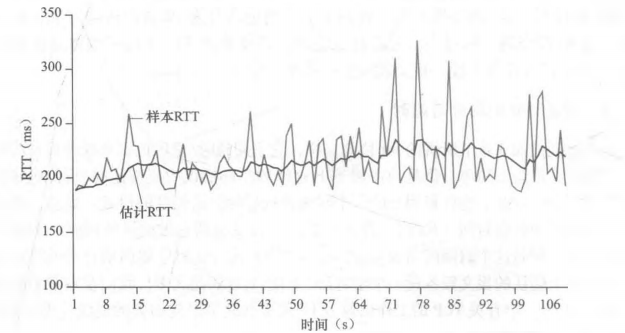
\includegraphics[width=0.6\textwidth]{image/chapter03/RTT样本与RTT估计.png}
    \caption{RTT样本与RTT估计}
\end{figure}

    [RFC 6298]定义了 RTT偏差DevRTT,用于估算SampleRTT 一般会偏离EstimatedRTT的程度:

$$
    DevRTT = (1 - \beta) \cdot DevRTT + \beta \cdot | SampleRTT - EstimatedRTT |
$$

    注意到DevRTT是一个SampleRTT与EstimatedRTT之间差值的EWMA\footnote[1]{从统计学观点讲,这种平均被称为指数加权移动平均(Exponential Weighted Moving Average, EWMA)。在 EWMA中的“指数” 一词看起来是指一个给定的SampleRTT的权值在更新的过程中呈指数型快速衰减。}。如果SampleRTT值波动较小,那么DevRTT的值就会很小;另一方面,如果波动很大,那么DevRTT的值就会很大。$\beta$的推荐值为0. 25。

\subsubsection{设置和管理重传超时间隔}

    假设已经给岀了EstimatedRTT值和DevRTT值,超时间隔应该大于等于EstimatedRTT,否则,将造成不必要的重传。但是超时间隔也不应该比EstimatedRTT大太多,否则当报文段丢失时,TCP不能很快地重传该报文段,导致数据传输时延大。

$$
    Timeoutinterval = EstimatedRTT + 4 \cdot DevRTT
$$

    推荐的初始Timeoutinterval值为1秒[RFC 6298]。同时,当出现超时后,TimeoutInterval值将加倍,以免即将被确认的后继报文段过早出现超时。然而,只要收到报文段并更新EstimatedRTT,就使用上述公式再次计算TimeoutInterva

\subsection{可靠数据传输}

    \emph{因特网的网络层服务(IP服务)是不可靠的。IP不保证数据报的交付,不保证数据报的按序交付,也不保证数据报中数据的完整性}。

    TCP在IP不可靠的尽力而为服务之上创建了一种可靠数据传输服务(reliable data transfer service)。TCP的可靠数据传输服务确保一个进程从其接收缓存中读出的数据流是无损坏、无间隙、非冗余和按序的数据流;即该字节流与连接的另一方端系统发送出的字节流是完全相同。

    我们将以两个递增的步骤来讨论TCP是如何提供可靠数据传输的。我们先给出一个TCP发送方的高度简化的描述,该发送方只用超时来恢复报文段的丢失;然后再给岀一个更全面的描述,该描述中除了使用超时机制外,还使用冗余确认技术。在接下来的讨论中,我们假定数据仅向一个方向发送,即从主机A到主机B,且主机A在发送一个大文件。

\begin{lstlisting}[language=C++, caption={简化的TCP发送方}]
/*
* 假设发送方不受TCP流量和拥塞控制的限制,来自上层数据的长度小于MSS,且数据传送只在一个
* 方向进行。
*/
NextSeqNum=InitialSeqNumber
SendBase=InitialSeqNumber

loop (永远) {
    switch (事件)
        事件:从上面应用程序接收到数据e
            生成具有序号NextSeqNum的TCP报文段
            if (定时器当前没有运行)
                启动定时器 
            向IP传递报文段
            NextSeqNum = NextSeqNum + length(data)
            break;
        事件:定时器超时
            重传具有最小序号但仍未应答的报文段
            启动定时器
            break;
        事件:收到ACK,具有ACK字段值y
            if (y > SendBase) {
                SendBase = y
                if (当前仍无任何应答报文段) {
                    启动定时器 
                }
            }
            break;
} /*结束永远循环*/
\end{lstlisting}

    我们看到在TCP发送方有3个与发送和重传有关的主要事件:从上层应用程序接收数据;定时器超时和收到ACK。

    一旦第一个主要事件发生,TCP从应用程序接收数据,将数据封装在一个报文段中,并把该报文段交给IP。

    还要注意到如果定时器还没有为某些其他报文段而运行,则当报文段被传给IP时,TCP就启动该定时器。(将定时器想象为与最早的未被确认的报文段相关联是有帮助的)。该定时器的过期间隔是Timeoutinterval\footnote[1]{由EstimatedRTT和DevRTT计算得出}

    第二个主要事件是超时。TCP通过重传引起超时的报文段来响应超时事件。然后TCP重启定时器。

    TCP发送方必须处理的第三个主要事件是,到达一个来自接收方的确认报文段(ACK)(更确切地说,是一个包含了有效ACK字段值的报文段)

\subsubsection{超时间隔加倍}

    在大多数TCP实现中所做的一些修改。首先关注的是在定时器时限过期后超时间隔的长度。在这种修改中,每当超时事件发生时,如前所述,TCP重传具有最小序号的还未被确认的报文段。只是每次TCP重传时都会将下一次的超时间隔设为先前值的两倍,而不是用从EstimatedRTT和DevRTT推算出的值

\subsubsection{快速重传}

    超时触发重传存在的问题之一是超时周期可能相对较长。当一个报文段丢失时,这种长超时周期迫使发送方延迟重传丢失的分组,因而增加了端到端时延。

    \emph{发送方通常可在超时事件发生之前通过注意所谓冗余ACK来较好地检测到丢包情况。冗余ACK(duplicate ACK)就是再次确认某个报文段的ACK,而发送方先前已经收到对该报文段的确认}。

\begin{figure}[!htbp]
    \centering
    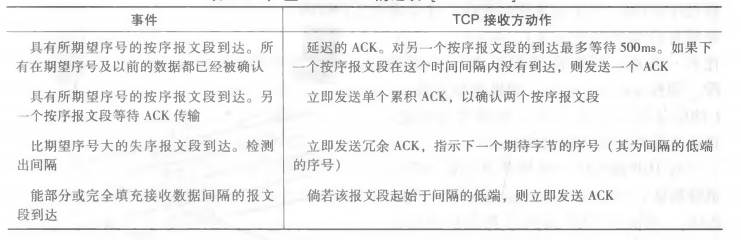
\includegraphics[width=0.6\textwidth]{image/chapter03/产生TCP ACK的建议.png}
    \caption{产生TCP ACK的建议 [RFC 5681]}
\end{figure}

    因为发送方经常一个接一个地发送大量的报文段,如果一个报文段丢失,就很可能引起许多一个接一个的冗余ACK。如果TCP发送方接收到对相同数据的3个冗余ACK,它把这当作一种指示,说明跟在这个已被确认过3次的报文段之后的报文段已经丢失。

    一旦收到3个冗余ACK, TCP就执行快速重传(fast retransmit)[ RFC 5681 ],即在该报文段的定时器过期之前重传丢失的报文段。对于采用快速重传的TCP,可用下列代码片段代替ACK收到事件: 

\begin{lstlisting}[language=C++, caption={针对快速重传的机制}]
事件:收到ACK,具有ACK字段值y
    if (y > SendBase) {
        SendBase=y
        if (当前仍无任何应答报文段)
            启动定时器
        }
    else {/* 快对已经确认的报文段的一个冗余ACK */
        对y收到的冗余ACK数加1
        if (对y == 3收到的冗余ACK数)
            /* TCP快速重传 */ 
            重新发送具有序号y的报文段
    }
    break;
\end{lstlisting}

\subsection{流量控制}

    \emph{一条TCP连接的每一侧主机都为该连接设置了接收缓存。当该TCP连接收到正确、按序的字节后,它就将数据放入接收缓存。相关联的应用进程会从该缓存中读取数据,但不必是数据刚一到达就立即读取}。

    TCP为它的应用程序提供了流量控制服务(flow control service)以消除发送方使接收方缓存溢岀的可能性。流量控制因此是一个速度匹配服务,即发送方的发送速率与接收方应用程序的读取速率相匹配。

    TCP发送方也可能因为IP网络的拥塞而被遏制;这种形式的发送方的控制被称为拥塞控制(congestion control)。

    值得注意的是:\emph{使流量控制和拥塞控制采取的动作非常相似(对发送方的遏制),但是它们显然是针对完全不同的原因而采取的措施。}

    TCP通过让发送方维护一个称为接收窗口(receive window)的变量来提供流量控制。通俗地说,接收窗口用于给发送方一个指示一一该接收方还有多少可用的缓存空间。\emph{因为TCP是全双工通信,在连接两端的发送方都各自维护一个接收窗口。}

    我们定义以下变量:

\begin{itemize}
    \item RcvBuffer:来表示接收缓存大小
    \item LastByteRead:主机B上的应用进程从缓存读出的数据流的最后一个字节的编号
    \item LastByteRcvd:从网络中到达的并且已放入主机B接收缓存中的数据流的最后一个字节的编号
\end{itemize}

    由于TCP不允许已分配的缓存溢岀,下式必须成立:

$$
    LastByteRcvd - LastByteRead = RcvBuffer
$$

    接收窗口用rwnd表示,根据缓存可用空间的数量来设置:

$$
    rwnd = RcvBuffer - [LastByteRcvd - LastByteRead]
$$

\begin{figure}[!htbp]
    \centering
    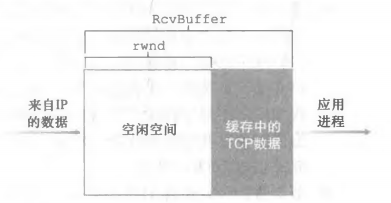
\includegraphics[width=0.6\textwidth]{image/chapter03/接收窗口和接收缓存.png}
    \caption{接收窗口和接收缓存}
\end{figure}

\subsection{TCP链接管理}

    TCP链接:

\begin{itemize}
    \item [1)] 客户端向服务器发送特殊TCP报文(也就是SYN报文段),此时SYN报文段被置1。然后随机选择初始序号$(client\_isn)$
    \item [2)] 当SYN报文段的IP数据包到达服务器主机,则提取出SYN,服务器端发送允许链接的报文段\footnote[1]{\emph{允许链接的报文段被称为SYNACK报文段(SYNACK segment)}}(此时,SYN同样包含,确认号字段为$client\_isn + 1$,最后服务器选择自己的初始序号$(server\_isn)$)
    \item [3)] 在收到SYNACK报文段后,客户给该链接分配缓存和变量。同时,向服务器发送链接确认的报文(SYN置0)
\end{itemize}

\begin{figure}[!htbp]
    \centering
    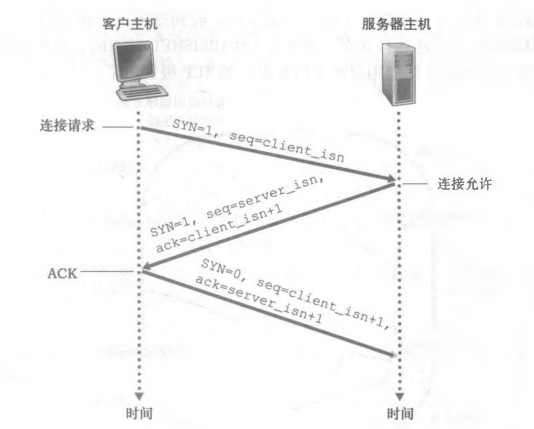
\includegraphics[width=0.6\textwidth]{image/chapter03/TCP三次握手,报文段交换.png}
    \caption{TCP三次握手:报文段交换}
\end{figure}

    当客户端发送关闭连接命令:

\begin{itemize}
    \item [1)] 客户端发送特殊TCP报文段(也就是FIN报文段)
    \item [2)] 服务器接收到FIN后,发送确认ACK报文段
    \item [3)] 服务器发送FIN终止报文段
    \item [4)] 客户端发送ACK确认报文段
\end{itemize}

    在一个TCP连接的生命周期内,运行在每台主机中的TCP协议在各种TCP状态(TCP state)之间变迁。

\begin{figure}[htbp]
    \begin{minipage}[t]{0.5\textwidth}
        \centering
        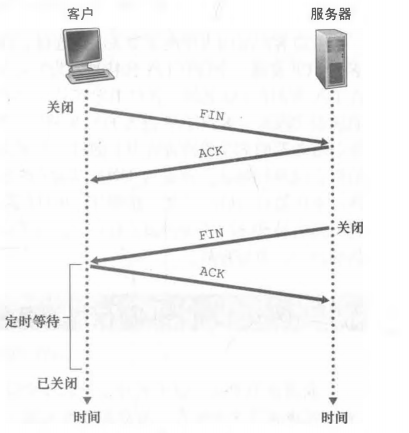
\includegraphics[width=\textwidth]{image/chapter03/TCP关闭连接.png}
        \caption{TCP关闭连接}
    \end{minipage}
    
    \begin{minipage}[t]{0.5\textwidth}
        \centering
        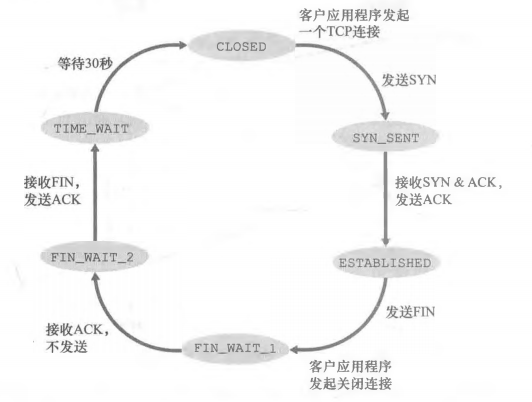
\includegraphics[width=\textwidth]{image/chapter03/TCP关闭状态.png}
        \caption{客户TCP经历的典型TCP状态序列}
    \end{minipage}    
\end{figure}

% \begin{figure}[!htbp]
    
% \end{figure}

    客户TCP开始时处于CLOSED(关闭)状态。客户的应用程序发起一个新的TCP连接。这引起客户中的TCP向服务器中的TCP发送一个SYN报文段。在发送过SYN报文段后,客户TCP进入了$SYN\_SENT$状态。

    当客户TCP处在$SYN\_SENT$状态时,它等待来自服务器TCP的对客户所发报文段进行确认且SYN比特被置为1的一个报文段。收到这样一个报文段之后,客户TCP进入ESTABLISHED(已建立)状态。

    当处在ESTABLISHED状态时,TCP客户就能发送和接收包含有效载荷数据(即应用层产生的数据)的TCP报文段了。

    假设客户应用程序决定要关闭该连接。这引起客户TCP发送一个带有FIN比特被置为1的TCP报文段,并进入$FIN\_WAIT\_1$状态。

    当处在$FIN\_WAIT\_1$状态时,客户TCP等待一个来自服务器的带有确认的TCP报文段。当它收到该报文段时,客户TCP进入$FIN\_WAIT\_2$状态。

    当处在$FIN\_WAIT\_2$状态时,客户等待来自服务器的FIN比特被置为1的另一个报文段;当收到该报文段后,客户TCP对服务器的报文段进行确认,并进入$TIME\_WAIT$状态。

    假定ACK丢失,$TIME\_WAIT$状态使TCP客户重传最后的确认报文。在$TIME\_WAIT$状态中所消耗的时间是与具体实现有关的,而典型的值是30秒、1分钟或2分钟。经过等待后,连接就正式关闭,客户端所有资源(包括端口号)将被释放。

    对于服务器TCP需要经历的流程:

\begin{figure}[!htbp]
    \centering
    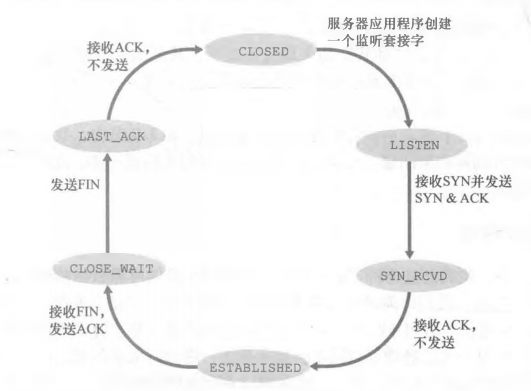
\includegraphics[width=0.6\textwidth]{image/chapter03/服务器TCP状态序列.png}
    \caption{服务器端TCP经历的典型TCP状态序列}
\end{figure}

\section{拥塞控制原理}

    在实践中,这种丢包一般是当网络变得拥塞时由于路由器缓存溢岀引起的。分组重传因此作为网络拥塞的征兆(某个特定的运输层报文段的丢失)来对待,但是却无法处理导致网络拥塞的原因,因为有太多的源想以过高的速率发送数据。为了处理网络拥塞原因,需要一些机制以在面临网络拥塞时遏制发送方

\subsection{拥塞原因与代价}

\subsubsection{情况一:两个发送方和一台具有无穷大缓存的路由器}

\begin{figure}[!htbp]
    \centering
    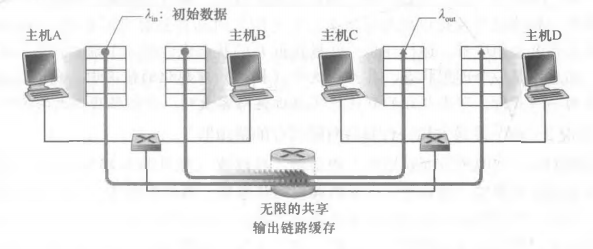
\includegraphics[width=0.6\textwidth]{image/chapter03/拥塞情况一.png}
    \caption{拥塞情况1:两条连接共享具有无限大缓存的单条路由}
\end{figure}

    假设主机A以$\lambda_{in}$字节/秒的平均速率发送数据到连接中,也就意味着主机A向路由器提供流量的速率是$\lambda_{in}$字节/秒。假设B也是如此,在一段容量为R的共享式输出链路上传输。因此,我们假设路由器有无限大的缓存空间。

    下图展示了主机A的连接性能

\begin{figure}[!htbp]
    \centering
    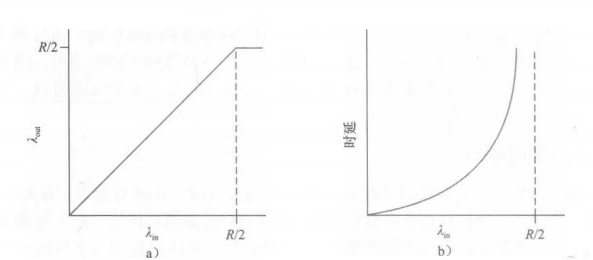
\includegraphics[width=0.6\textwidth]{image/chapter03/拥塞情况一吞吐量与延时等关系.png}
    \caption{拥塞情况1:吞吐量、时延与主机发送速率的函数关系}
\end{figure}

    可以看见,在发送速率为$0 ~ R/2$之间时,接收方的吞吐量等于发送方的发送速率;然而当越过R/2时,吞吐量只能到达R/2,无论如何也不会超过。

    并且,在无限接近R/2时,平均时延会趋向于无穷大,因此:\emph{即当分组的到达速率接近链路容量时,分组经历巨大的排队时延}

\subsubsection{情况2:两个发送方和一台具有有限缓存的路由器}

    在情况一的基础上进行修正:从无限缓存变为有限。当分组到达一个已满的缓存时会被丢弃。其次,我们假定每条连接都是可靠的。如果一个包含有运输层报文段的分组在路由器中被丢弃,那么它终将被发送方重传。

    我们再次以$\lambda_{in}$字节/秒表示应用程序将初始数据发送到套接字中的速率。运输层向网络中发送报文段(含有初始数据或重传数据)的速率用$\lambda_{in}^{'}$;字节/秒表示。$\lambda_{in}^{'}$有时被称为网络的供给载荷(offered load)。

\begin{figure}[!htbp]
    \centering
    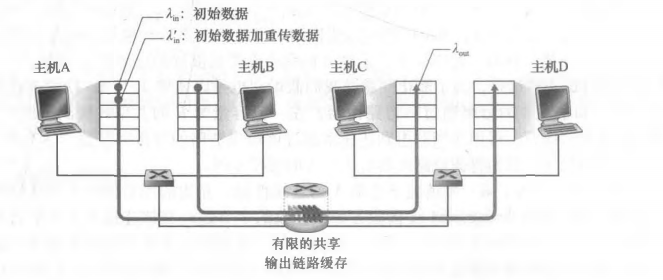
\includegraphics[width=0.6\textwidth]{image/chapter03/拥塞情况二.png}
    \caption{情况2:(有重传的)两台主机与一台拥有有限缓存的路由器}
\end{figure}

    在情况2下实现的性能强烈地依赖于重传的方式。

    首先考虑一种假设:主机A能够确定路由器中的缓存是否有空闲,因此只会在空闲时发送分组。这种情况下不会产生丢包并且$\lambda_{in} = \lambda_{out}$,连接的吞吐量就等于$\lambda_{in}$。如下图中图a所示

    于是考虑一种更为真实的情况:发送方仅当确认了一个分组丢失才会重传。由图b所示,\emph{发送方必须执行重传以补偿因为缓存溢出而丢弃(丢失)的分组}

    最后,我们考虑:发送方也许会提前发送超时并重传在队列中已被推迟但未丢失的分组。如图c所示,\emph{发送方在遇到大时延时所进行的不必要重传会引起路由器利用其链路带宽来转发不必要的分组副本}

\begin{figure}[!htbp]
    \centering
    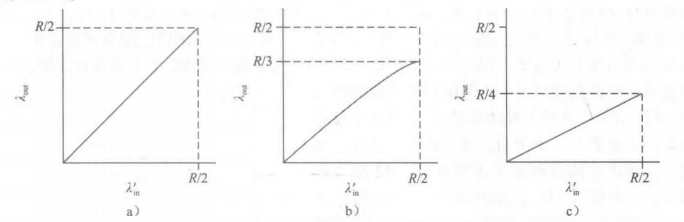
\includegraphics[width=0.8\textwidth]{image/chapter03/拥塞情况二吞吐量与延时等关系.png}
    \caption{具有有限缓存时情况2的性能}
\end{figure}

\subsection{拥塞控制方法}

    在最为宽泛的级别上,我们可根据网络层是否为运输层拥塞控制提供了显式帮助,来区分拥塞控制方法

\begin{itemize}
    \item [1)] 端到端拥寒控制。
    \subitem 在该方法中,网络层并没有为运输层拥塞控制提供显示支持。
    \item [2)] 网络辅助的拥塞控制
    \subitem 在该方法中,路由器向发送方提供关于网络中拥塞状态的显示反馈信息
\end{itemize}

